\documentclass[aspectratio=169,xcolor={usenames,dvipsnames}]{beamer}
% Handout Parameter, um die Foliensätze ohne einzelne "Klick-Schritte" zu generieren
%\documentclass[aspectratio=169,xcolor={usenames,dvipsnames}, handout]{beamer}
\usepackage[utf8x]{inputenc}
\usepackage[T1]{fontenc}
\usepackage{lmodern}
\usepackage[ngerman]{babel}
\usepackage{multimedia}
\usepackage{longtable}
\usepackage{array}
\usepackage{tikz}
\usepackage{listings}
\usepackage{caption}
\usepackage{transparent}
 
\usetheme{Szeged}

\beamertemplatenavigationsymbolsempty

\title{Mein Arbeitstitel}
\author{Micky Maus}
\institute{Seminar - Disneys Hochschule}


\useoutertheme[footline=institutetitle]{miniframes}
\setbeamercolor{separation line}{use=structure,bg=structure.fg!50!bg}
\DeclareCaptionFont{white}{\color{white}}
\DeclareCaptionFormat{listing}{\colorbox{gray}{\parbox{\textwidth}{#1#2#3}}}
\captionsetup[lstlisting]{format=listing,labelfont=white,textfont=white}

\begin{document}

% Angepasster Footer mit Seitenzahlen (aktuell und max)
\setbeamertemplate{footline}
{
  \begin{beamercolorbox}[colsep=1.5pt]{upper separation line foot}
  \end{beamercolorbox}
\hbox{
\begin{beamercolorbox}[wd=0.5\paperwidth, ht=2.5ex, dp=1.125ex, left]{title in head/foot}
      \usebeamerfont{title in head/foot}\insertshorttitle
    \end{beamercolorbox}
\raggedright
\begin{beamercolorbox}[wd=0.5\paperwidth, ht=2.5ex, dp=1.125ex, right]{title in head/foot}
      \usebeamerfont{title in head/foot}\insertframenumber/\inserttotalframenumber\hspace*{2ex}
\end{beamercolorbox}
}
 \begin{beamercolorbox}[colsep=1.5pt]{lower separation line foot}
  \end{beamercolorbox}
}

% Strukturfarbe
\definecolor{flocksserver}{RGB}{0,100,0}

\setbeamercolor{normal text}{fg=black,bg=white}
\setbeamercolor{alerted text}{fg=red}
\setbeamercolor{example text}{fg=green!50!black}

\setbeamercolor{structure}{fg=flocksserver}
%\setbeamercolor{structure}{fg=Bittersweet}

\setbeamercolor{background canvas}{parent=normal text}
\setbeamercolor{background}{parent=background canvas}

\setbeamercolor{palette primary}{fg=yellow,bg=yellow} % changed this
\setbeamercolor{palette secondary}{use=structure,fg=structure.fg!100!green} % changed this
\setbeamercolor{palette tertiary}{use=structure,fg=structure.fg!100!green} % changed this


\begin{frame}
\titlepage
\end{frame}
\begin{frame}
\frametitle{Übersicht}
\tableofcontents
\end{frame}
\section{Einleitung}

\subsection*{Einleitung}

\begin{frame}
	\frametitle{Vorwissen?}
		\begin{figure}[ht]
			
\includegraphics[width=6.5cm]{Bilder/fragerunde.png}
		\end{figure}
\end{frame}

\begin{frame}
	\frametitle{Was kann ich von dem Vortrag erwarten?}
	\begin{itemize}[<+->]
		\item Erster Punkt \emph{wichtig}
		\item Zweiter Punkt
		\item Dritter Punkt
	\end{itemize}
\end{frame}

\section{Hauptteil}

\subsection*{Hauptteil}

\begin{frame}
	\frametitle{Eine tolle Überschrift}
	\begin{columns}[c]
		\column[c]{5.6cm}
		\begin{exampleblock}{Block}
			\glqq Dies ist nur die Aussage der Präsentation und nicht zwingend die Meinung des Autors\grqq
		\end{exampleblock}
		\column{8cm}
		\begin{figure}[ht]
			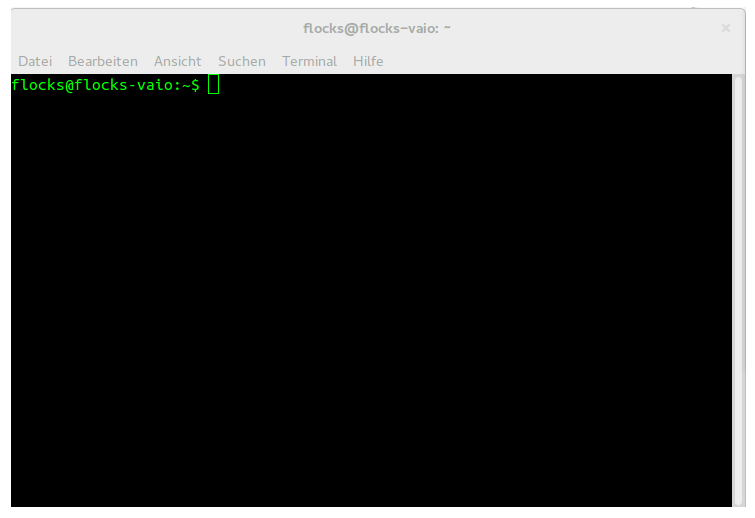
\includegraphics[width=7cm]{Bilder/bild.png}\caption{Toller Screenshot}
		\end{figure}
	\end{columns}
\end{frame}

\section{Schluss}

\subsection*{Schluss}

\begin{frame}
	\frametitle{Fazit}
	\begin{itemize}[<+->]
		\item Erster Punkt \emph{wichtig}
		\item Zweiter Punkt
		\item Dritter Punkt
	\end{itemize}
\end{frame}

\begin{frame}
	\frametitle{Fragen und Antworten}
	\begin{figure}[ht]
		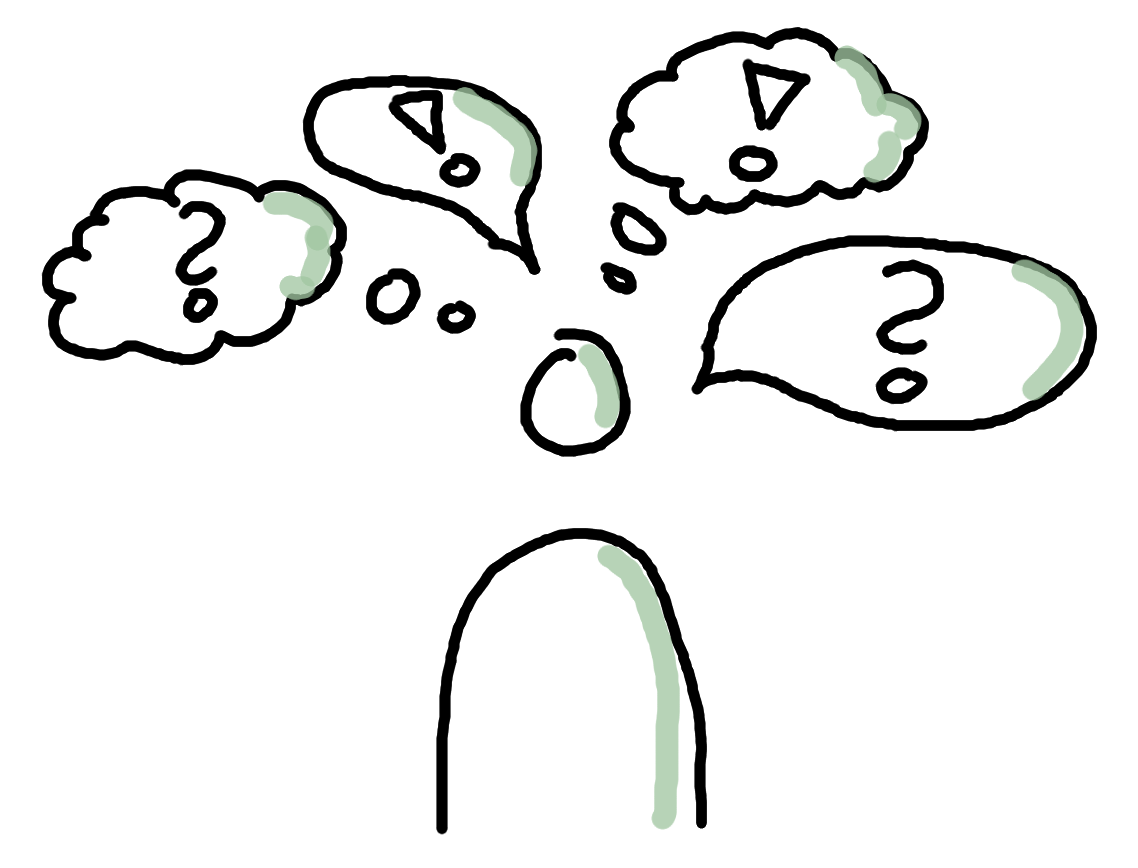
\includegraphics[width=8.0cm]{Bilder/fragenantwort.png}
	\end{figure}
\end{frame}
\begin{frame}[allowframebreaks]
	\frametitle{Quellen}
	\begin{thebibliography}{1}
		\bibitem{hp:marcel1}
		Marcel Kaufmann, \emph{TTVN Wechselliste Saison 2015/2016}, \url{http://flocksserver.de/\#projektVHCI}, Aufruf: 16.09.2015 14:18 Uhr. \hskip 1em plus
		0.5em minus 0.4em
		
		\bibitem{hp:marcel2}
		Marcel Kaufmann, \emph{NFC-Hack}, \url{http://flocksserver.de/\#projektNFC}, Aufruf: 16.09.2015 14:18 Uhr. \hskip 1em plus
		0.5em minus 0.4em
		
		\bibitem{hp:marcel3}
		Flocksserver, \emph{Youtube Channel}, \url{http://flocksserver.de/\#projektYoutube}, Aufruf: 16.09.2015 14:18 Uhr. \hskip 1em plus
		0.5em minus 0.4em
		
		\bibitem{hp:marcel4}
		Flocksserver, \emph{Homepage}, \url{http://flocksserver.de}, Aufruf: 16.09.2015 14:18 Uhr. \hskip 1em plus
		0.5em minus 0.4em
		
		\bibitem{hp:marcel5}
		Marcel Kaufmann, \emph{Tischtennis - Übungen visualisieren}, \url{http://flocksserver.de/\#projektTTVIS}, Aufruf: 16.09.2015 14:18 Uhr. \hskip 1em plus
		0.5em minus 0.4em
		
		\bibitem{hp:marcel6}
		Marcel Kaufmann, \emph{XING Profil Marcel Kaufmann}, \url{https://www.xing.com/profile/Marcel_Kaufmann24}, Aufruf: 16.09.2015 14:18 Uhr. \hskip 1em plus
		0.5em minus 0.4em
		
		\bibitem{hp:marcel6}
		Marcel Kaufmann, \emph{Youtube Channel Marcel Kaufmann}, \url{https://www.youtube.com/channel/UCde9DdEoqtM_Qf8s8YQRQvQ}, Aufruf: 16.09.2015 14:18 Uhr. \hskip 1em plus
		0.5em minus 0.4em
		
	\end{thebibliography}
\end{frame}



\end{document}